\IfFileExists{stacks-project.cls}{%
\documentclass{stacks-project}
}{%
\documentclass{amsart}
}
\usepackage{amssymb}

% For dealing with references we use the comment environment
\usepackage{verbatim}
\usepackage{fancyvrb}
\usepackage{pmboxdraw}
\newenvironment{reference}{\comment}{\endcomment}
%\newenvironment{reference}{}{}
\newenvironment{slogan}{\comment}{\endcomment}
\newenvironment{history}{\comment}{\endcomment}

% For source figures retained as assets
\usepackage{graphicx}

% For commutative diagrams we use Xy-pic
\usepackage[all]{xy}

% We use 2cell for 2-commutative diagrams.
\xyoption{2cell}
\UseAllTwocells

% We use multicol for the list of chapters between chapters
\usepackage{multicol}

% This is generally recommended for better output
\usepackage{lmodern}
\usepackage[T1]{fontenc}
\usepackage{textalpha}

% For cross-file-references
% We prefer the snapshot tmp/xref/#2.aux,
% which latexmkrc replaces atomically, so
% that documents compiled simultaneously
% never read a half-written .aux file.
% The last argument keeps links to #2.pdf.
\usepackage{xr-hyper}
\newcommand{\maybeexternaldocument}[2]{%
  \IfFileExists{#2.aux}{%
    \externaldocument[#1]{#2}%
  }{%
    \PackageWarning{stack}{Missing #2.aux; external references with prefix #1 unavailable}%
  }%
}
\let\externaldocumentorig\externaldocument
\renewcommand{\externaldocument}[2][]{%
  \IfFileExists{tmp/xref/#2.aux}{%
    \externaldocumentorig[#1]{tmp/xref/#2}[#2.pdf]%
  }{%
  \IfFileExists{#2.aux}{%
    \externaldocumentorig[#1]{#2}%
  }{%
    \PackageWarning{stack}{Missing #2.aux; external references with prefix #1 unavailable}%
  }%
  }%
}

% Package for hypertext links:
\usepackage{hyperref}

% For any local file, say "hello.tex" you want to link to please
% use \externaldocument[hello-]{hello}
\externaldocument[introduction-]{introduction}
\externaldocument[conventions-]{conventions}
\externaldocument[sets-]{sets}
\externaldocument[categories-]{categories}
\externaldocument[topology-]{topology}
\externaldocument[sheaves-]{sheaves}
\externaldocument[sites-]{sites}
\externaldocument[stacks-]{stacks}
\externaldocument[fields-]{fields}
\externaldocument[algebra-]{algebra}
\externaldocument[brauer-]{brauer}
\externaldocument[homology-]{homology}
\externaldocument[derived-]{derived}
\externaldocument[simplicial-]{simplicial}
\externaldocument[more-algebra-]{more-algebra}
\externaldocument[smoothing-]{smoothing}
\externaldocument[modules-]{modules}
\externaldocument[sites-modules-]{sites-modules}
\externaldocument[injectives-]{injectives}
\externaldocument[cohomology-]{cohomology}
\externaldocument[sites-cohomology-]{sites-cohomology}
\externaldocument[dga-]{dga}
\externaldocument[dpa-]{dpa}
\externaldocument[sdga-]{sdga}
\externaldocument[hypercovering-]{hypercovering}
\externaldocument[schemes-]{schemes}
\externaldocument[constructions-]{constructions}
\externaldocument[properties-]{properties}
\externaldocument[morphisms-]{morphisms}
\externaldocument[coherent-]{coherent}
\externaldocument[divisors-]{divisors}
\externaldocument[limits-]{limits}
\externaldocument[varieties-]{varieties}
\externaldocument[topologies-]{topologies}
\externaldocument[descent-]{descent}
\externaldocument[perfect-]{perfect}
\externaldocument[more-morphisms-]{more-morphisms}
\externaldocument[flat-]{flat}
\externaldocument[groupoids-]{groupoids}
\externaldocument[more-groupoids-]{more-groupoids}
\externaldocument[etale-]{etale}
\externaldocument[chow-]{chow}
\externaldocument[intersection-]{intersection}
\externaldocument[pic-]{pic}
\externaldocument[weil-]{weil}
\externaldocument[adequate-]{adequate}
\externaldocument[dualizing-]{dualizing}
\externaldocument[duality-]{duality}
\externaldocument[discriminant-]{discriminant}
\externaldocument[derham-]{derham}
\externaldocument[local-cohomology-]{local-cohomology}
\externaldocument[algebraization-]{algebraization}
\externaldocument[curves-]{curves}
\externaldocument[resolve-]{resolve}
\externaldocument[models-]{models}
\externaldocument[functors-]{functors}
\externaldocument[equiv-]{equiv}
\externaldocument[pione-]{pione}
\externaldocument[etale-cohomology-]{etale-cohomology}
\externaldocument[proetale-]{proetale}
\externaldocument[relative-cycles-]{relative-cycles}
\externaldocument[more-etale-]{more-etale}
\externaldocument[trace-]{trace}
\externaldocument[crystalline-]{crystalline}
\externaldocument[spaces-]{spaces}
\externaldocument[spaces-properties-]{spaces-properties}
\externaldocument[spaces-morphisms-]{spaces-morphisms}
\externaldocument[decent-spaces-]{decent-spaces}
\externaldocument[spaces-cohomology-]{spaces-cohomology}
\externaldocument[spaces-limits-]{spaces-limits}
\externaldocument[spaces-divisors-]{spaces-divisors}
\externaldocument[spaces-over-fields-]{spaces-over-fields}
\externaldocument[spaces-topologies-]{spaces-topologies}
\externaldocument[spaces-descent-]{spaces-descent}
\externaldocument[spaces-perfect-]{spaces-perfect}
\externaldocument[spaces-more-morphisms-]{spaces-more-morphisms}
\externaldocument[spaces-flat-]{spaces-flat}
\externaldocument[spaces-groupoids-]{spaces-groupoids}
\externaldocument[spaces-more-groupoids-]{spaces-more-groupoids}
\externaldocument[bootstrap-]{bootstrap}
\externaldocument[spaces-pushouts-]{spaces-pushouts}
\externaldocument[spaces-chow-]{spaces-chow}
\externaldocument[groupoids-quotients-]{groupoids-quotients}
\externaldocument[spaces-more-cohomology-]{spaces-more-cohomology}
\externaldocument[spaces-simplicial-]{spaces-simplicial}
\externaldocument[spaces-duality-]{spaces-duality}
\externaldocument[formal-spaces-]{formal-spaces}
\externaldocument[restricted-]{restricted}
\externaldocument[spaces-resolve-]{spaces-resolve}
\externaldocument[formal-defos-]{formal-defos}
\externaldocument[defos-]{defos}
\externaldocument[cotangent-]{cotangent}
\externaldocument[examples-defos-]{examples-defos}
\externaldocument[algebraic-]{algebraic}
\externaldocument[examples-stacks-]{examples-stacks}
\externaldocument[stacks-sheaves-]{stacks-sheaves}
\externaldocument[criteria-]{criteria}
\externaldocument[artin-]{artin}
\externaldocument[quot-]{quot}
\externaldocument[stacks-properties-]{stacks-properties}
\externaldocument[stacks-morphisms-]{stacks-morphisms}
\externaldocument[stacks-limits-]{stacks-limits}
\externaldocument[stacks-cohomology-]{stacks-cohomology}
\externaldocument[stacks-perfect-]{stacks-perfect}
\externaldocument[stacks-introduction-]{stacks-introduction}
\externaldocument[stacks-more-morphisms-]{stacks-more-morphisms}
\externaldocument[stacks-geometry-]{stacks-geometry}
\externaldocument[moduli-]{moduli}
\externaldocument[moduli-curves-]{moduli-curves}
\externaldocument[examples-]{examples}
\externaldocument[exercises-]{exercises}
\externaldocument[guide-]{guide}
\externaldocument[desirables-]{desirables}
\externaldocument[coding-]{coding}
\externaldocument[obsolete-]{obsolete}
\externaldocument[fdl-]{fdl}
\externaldocument[index-]{index}

% Heap Project documents
\externaldocument[k3-]{k3}
\externaldocument[torelli-]{torelli}
\externaldocument[linear-algebra-]{linear-algebra}
\externaldocument[groups-]{groups}
\externaldocument[complex-analysis-]{complex-analysis}
\externaldocument[functional-analysis-]{functional-analysis}
\externaldocument[categories-]{categories}
\externaldocument[commutative-algebra-]{commutative-algebra}
\externaldocument[ringed-spaces-]{ringed-spaces}
\externaldocument[homological-algebra-]{homological-algebra}
\externaldocument[lie-algebras-]{lie-algebras}
\externaldocument[representation-theory-]{representation-theory}
\externaldocument[smooth-manifolds-]{smooth-manifolds}
\externaldocument[differential-topology-]{differential-topology}
\externaldocument[algebraic-topology-]{algebraic-topology}
\externaldocument[differential-geometry-]{differential-geometry}
\externaldocument[algebraic-geometry-]{algebraic-geometry}
\externaldocument[symplectic-geometry-]{symplectic-geometry}
\externaldocument[complex-geometry-]{complex-geometry}
\externaldocument[hodge-theory-]{hodge-theory}
\externaldocument[%
variations-of-hodge-structures-]{%
variations-of-hodge-structures}
\externaldocument[%
homological-mirror-symmetry-]{%
homological-mirror-symmetry}
\maybeexternaldocument{deformations-}{deformations}
\externaldocument[vertex-algebras-]{vertex-algebras}
\externaldocument[springer-]{springer}
\externaldocument[infty-categories-]{infty-categories}
\externaldocument[seminars-differential-geometry-]{%
seminars-differential-geometry}
\externaldocument[seminars-complex-geometry-]{%
seminars-complex-geometry}
\externaldocument[seminars-algebraic-geometry-]{%
seminars-algebraic-geometry}
\externaldocument[seminars-analysis-pde-]{%
seminars-analysis-pde}
\externaldocument[surfaces-]{surfaces}
\externaldocument[birational-maps-commutative-algebra-]{birational-maps-commutative-algebra}
\externaldocument[cremona-transformations-]{cremona-transformations}
\externaldocument[derived-categories-of-sheaves-]{derived-categories-of-sheaves}
\externaldocument[geometric-invariant-theory-]{geometric-invariant-theory}
\externaldocument[geometric-stability-conditions-and-group-actions-]{geometric-stability-conditions-and-group-actions}
\externaldocument[moduli-spaces-of-sheaves-]{moduli-spaces-of-sheaves}
\externaldocument[bridgeland-stability-general-theory-]{bridgeland-stability-general-theory}
\externaldocument[hilbert-schemes-]{hilbert-schemes}
\externaldocument[noncommutative-abelian-surfaces-and-kummer-type-hyperkahler-varieties-]{noncommutative-abelian-surfaces-and-kummer-type-hyperkahler-varieties}
\externaldocument[mumford-tate-groups-in-hodge-theory-]{mumford-tate-groups-in-hodge-theory}
\externaldocument[hodge-birational-atoms-2026-]{hodge-birational-atoms-2026}
\externaldocument[xxii-egd-2026-]{%
xxii-egd-2026}
\externaldocument[pde-]{pde}
\externaldocument[probability-]{probability}

\externaldocument[linguistics-]{linguistics}

\externaldocument[%
16th-alga-meeting-2026-]{%
16th-alga-meeting-2026}

\externaldocument[%
iv-jornadas-lefschetz-2026-]{%
iv-jornadas-lefschetz-2026}

\externaldocument[reading-the-masters-]{%
reading-the-masters}

\externaldocument[real-analysis-]{%
real-analysis}

\externaldocument[optimal-transport-]{%
optimal-transport}

\externaldocument[history-]{history}

\externaldocument[seiberg-witten-]{seiberg-witten}

\externaldocument[history-philosophy-biology-]{history-philosophy-biology}

\externaldocument[classical-mechanics-]{classical-mechanics}
\externaldocument[electromagnetism-]{electromagnetism}
\externaldocument[waves-and-optics-]{waves-and-optics}
\externaldocument[wif-]{waves-in-fluids-iv}
\externaldocument[thermal-physics-]{thermal-physics}
\externaldocument[quantum-mechanics-]{quantum-mechanics}
\externaldocument[special-relativity-]{special-relativity}
\externaldocument[physics-]{physics}

\externaldocument[chemistry-]{chemistry}

\externaldocument[molecular-cell-biology-]{molecular-cell-biology}

\externaldocument[microbiology-]{microbiology}

\externaldocument[protistology-]{protistology}

\externaldocument[mycology-]{mycology}

\externaldocument[botany-]{botany}

\externaldocument[zoology-]{zoology}

\externaldocument[animal-histology-]{animal-histology}

\externaldocument[animal-physiology-]{animal-physiology}

\externaldocument[systematics-biogeography-]{systematics-biogeography}

\externaldocument[ecology-natural-resources-]{ecology-natural-resources}

\externaldocument[earth-sciences-]{earth-sciences}

\externaldocument[biostatistics-]{biostatistics}

\externaldocument[mathematical-systems-biology-]{mathematical-systems-biology}

\externaldocument[cimpa-el-salvador-2024-]{cimpa-el-salvador-2024}

\externaldocument[anthropology-]{anthropology}

\externaldocument[yang-mills-theory-]{yang-mills-theory}

\externaldocument[seminars-algebra-]{seminars-algebra}

\externaldocument[seminars-physics-]{seminars-physics}

\externaldocument[seminars-computing-]{seminars-computing}

\externaldocument[oktobermat-2026-]{oktobermat-2026}

\externaldocument[saet-2026-]{saet-2026}

\externaldocument[seminars-symplectic-geometry-]{seminars-symplectic-geometry}

\externaldocument[seminars-dynamics-]{seminars-dynamics}

\externaldocument[oktobermat-2024-]{oktobermat-2024}

\externaldocument[quantum-groups-]{quantum-groups}

\externaldocument[legal-2027-]{legal-2027}

\externaldocument[derived-categories-]{derived-categories}

% Theorem environments.
%
\theoremstyle{plain}
\newtheorem{theorem}[subsection]{Theorem}
\newtheorem{proposition}[subsection]{Proposition}
\newtheorem{lemma}[subsection]{Lemma}
\newtheorem{corollary}[subsection]{Corollary}

\theoremstyle{definition}
\newtheorem{definition}[subsection]{Definition}
\newtheorem{example}[subsection]{Example}
\newtheorem{exercise}[subsection]{Exercise}
\newtheorem{situation}[subsection]{Situation}

\theoremstyle{remark}
\newtheorem{remark}[subsection]{Remark}
\newtheorem{remarks}[subsection]{Remarks}

\numberwithin{equation}{subsection}

% Macros
%
\def\lim{\mathop{\mathrm{lim}}\nolimits}
\def\colim{\mathop{\mathrm{colim}}\nolimits}
\def\Spec{\mathop{\mathrm{Spec}}}
\def\Hom{\mathop{\mathrm{Hom}}\nolimits}
\def\Ext{\mathop{\mathrm{Ext}}\nolimits}
\def\SheafHom{\mathop{\mathcal{H}\!\mathit{om}}\nolimits}
\def\SheafExt{\mathop{\mathcal{E}\!\mathit{xt}}\nolimits}
\def\Sch{\mathit{Sch}}
\def\Mor{\mathop{\mathrm{Mor}}\nolimits}
\def\Ob{\mathop{\mathrm{Ob}}\nolimits}
\def\Sh{\mathop{\mathit{Sh}}\nolimits}
\def\NL{\mathop{N\!L}\nolimits}
\def\CH{\mathop{\mathrm{CH}}\nolimits}
\def\proetale{{pro\text{-}\acute{e}tale}}
\def\etale{{\acute{e}tale}}
\def\QCoh{\mathit{QCoh}}
\def\Ker{\mathop{\mathrm{Ker}}}
\def\Im{\mathop{\mathrm{Im}}}
\def\Coker{\mathop{\mathrm{Coker}}}
\def\Coim{\mathop{\mathrm{Coim}}}

% Boxtimes
%
\DeclareMathSymbol{\boxtimes}{\mathbin}{AMSa}{"02}

%
% Macros for moduli stacks/spaces
%
\def\QCohstack{\mathcal{QC}\!\mathit{oh}}
\def\Cohstack{\mathcal{C}\!\mathit{oh}}
\def\Spacesstack{\mathcal{S}\!\mathit{paces}}
\def\Quotfunctor{\mathrm{Quot}}
\def\Hilbfunctor{\mathrm{Hilb}}
\def\Curvesstack{\mathcal{C}\!\mathit{urves}}
\def\Polarizedstack{\mathcal{P}\!\mathit{olarized}}
\def\Complexesstack{\mathcal{C}\!\mathit{omplexes}}
% \Pic is the operator that assigns to X its picard group, usage \Pic(X)
% \Picardstack_{X/B} denotes the Picard stack of X over B
% \Picardfunctor_{X/B} denotes the Picard functor of X over B
\def\Pic{\mathop{\mathrm{Pic}}\nolimits}
\def\Picardstack{\mathcal{P}\!\mathit{ic}}
\def\Picardfunctor{\mathrm{Pic}}
\def\Deformationcategory{\mathcal{D}\!\mathit{ef}}


\begin{document}

\title{Knot Theory}
\maketitle

\phantomsection
\label{section-phantom}

\tableofcontents

\section{Overview}
\label{section-overview}

\noindent
These notes bring back the basics of two
knot theory courses I took at UNAM: the
Seminario de Topolog\'ia A (Teor\'ia de
nudos y aplicaciones) of 2020 and the
Seminario de Topolog\'ia B that followed
it. They are a small chapter of basics,
written from my old course files and
from textbooks.

\medskip\noindent
{\bf Sources.} My course files. They are exercise
sheets, short typed notes of the
teachers and my handwritten solutions;
there are no full lecture notes among
them. The sheet of my Ejercicio 2 for
Seminario de Topolog\'ia B names the
lecturer as Dr.\ Vinicio Antonio G\'omez
Guti\'errez. The typed notes of the
first course refer to a lecturer
``Dr.\ Jos\'e Carlos''; no file that I
read gives his surname or the author of
those notes. The statements and the
numbering are taken from the books
\cite{murasugi}, \cite{lickorish},
\cite{adams-knot-book} and
\cite{hatcher}. The notation
$K_{q,r}$ of my exercises is that of
\cite[Chapter 7]{murasugi}, so the
course followed that book at least for
torus knots. Whenever a statement comes
from a course file I name the file.

\medskip\noindent
{\bf Big picture.} A knot is a closed
curve in space. Two knots are the same
when one can be deformed into the other
without cutting. The subject is the
search for {\it invariants}: quantities
computed from a picture of the knot that
do not change under deformation, so that
different values prove that two knots
are different. The steps are:
\begin{enumerate}
\item Replace the knot by a planar
picture, a diagram
(Section \ref{section-knots-diagrams}).
\item Reduce deformations of the knot to
three local changes of the diagram, the
Reidemeister moves
(Section \ref{section-reidemeister}).
An invariant is then anything unchanged
by the three moves.
\item First invariants: the linking
number and three-colourings
(Sections \ref{section-linking-number}
and \ref{section-three-colourings}).
\item The Kauffman bracket is unchanged
by two of the three moves; correcting it
by the writhe gives the Jones polynomial
(Sections \ref{section-kauffman-bracket}
and \ref{section-jones-polynomial}).
The trefoil is computed in full in
Section \ref{section-trefoil}, and
Section \ref{section-chirality} uses it
to tell the trefoil from its mirror
image.
\item Torus knots are the curves of
class $(p,q)$ on a torus in the
three-sphere
(Sections \ref{section-curves-on-torus}
and \ref{section-torus-knots}).
\item The fundamental group of the
complement, computed with van Kampen's
theorem
(Section \ref{section-knot-group}), and
the Alexander polynomial
(Section \ref{section-alexander}).
\end{enumerate}
The computations of
Section \ref{section-trefoil} are
checked by an exact computer script.
It is the file
{\tt check\_knot\_jones.py} in the
folder {\tt scripts}.

\section{Knots, links and diagrams}
\label{section-knots-diagrams}

\noindent
A {\it knot} is a subset $K$ of
$\mathbb{R}^3$ that is the image of an
injective continuous map from the circle
$S^1$ to $\mathbb{R}^3$. We always
assume that $K$ is a closed polygon with
finitely many edges, or a smooth curve
with nowhere vanishing velocity; this
excludes pathological (``wild'') curves.
A {\it link} is a union of finitely many
pairwise disjoint knots, called its
{\it components}. A knot is a link with
one component. A link is {\it oriented}
when a direction of travel is chosen on
each component.

\medskip\noindent
Two links $L$ and $L'$ are
{\it equivalent} if there is an
orientation-preserving homeomorphism of
$\mathbb{R}^3$ that maps $L$ onto $L'$.
This is
\cite[Definition 1.3.1]{murasugi}. For
oriented links the homeomorphism must
also respect the directions. It makes no
difference to work in the three-sphere
$S^3$, which is $\mathbb{R}^3$ with one
point added at infinity.

\medskip\noindent
The {\it trivial knot} or {\it unknot}
is the round circle in a plane, and any
knot equivalent to it. The {\it trivial
link} with $c$ components is a union of
$c$ disjoint round circles in a plane,
none inside another.

\medskip\noindent
A {\it diagram} of a link $L$ is its
image under the projection
$(x,y,z)\mapsto(x,y)$ to the plane,
when this image has only finitely many
multiple points, each of them a point
where exactly two pieces of the link
cross at a nonzero angle, together with
the information, at each such
{\it crossing}, of which piece is above
(has larger $z$). The piece above is the
{\it over-strand}, the other one the
{\it under-strand}. In pictures the
under-strand is drawn broken. After a
small rotation every link has a diagram.
An {\it arc} of a diagram is a piece of
the picture that runs from one break to
the next one.

\section{Reidemeister moves}
\label{section-reidemeister}

\noindent
The three {\it Reidemeister moves}
change a diagram inside a small disc and
leave the rest untouched.
\begin{center}
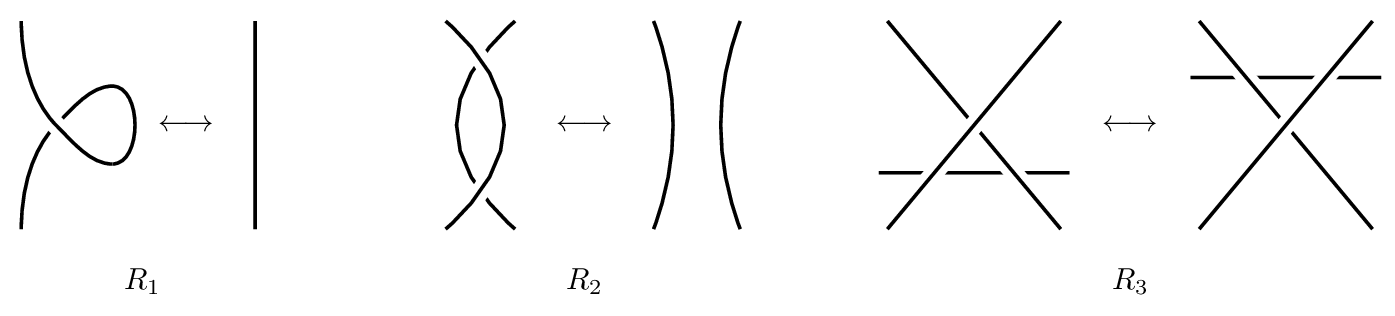
\includegraphics[width=.95\textwidth]{
knot-theory-assets/reidemeister.png}
\end{center}
The move $R_1$ adds or removes a
{\it kink}, that is, a small loop with
one crossing. The move $R_2$ slides one
strand over another, which creates or
removes two crossings. The move $R_3$
slides a strand across a crossing of two
other strands. Each move comes also in
its mirror versions, with over and under
exchanged.

\begin{theorem}[Reidemeister]
\label{theorem-reidemeister}
Let $D$ and $D'$ be diagrams of the
links $L$ and $L'$. Then $L$ and $L'$
are equivalent if and only if $D'$ is
obtained from $D$ by a finite sequence
of moves $R_1$, $R_2$, $R_3$, their
inverses, and deformations of the plane
that do not change the crossings.
\end{theorem}

\begin{proof}
See \cite[Theorem 4.1.1]{murasugi}.
\end{proof}

\noindent
So, to define an invariant of links it
is enough to define a quantity on
diagrams and to check that each of the
three moves leaves it unchanged. This is
how every invariant below is obtained,
except the knot group.

\section{Linking number and writhe}
\label{section-linking-number}

\noindent
Let $D$ be a diagram of an oriented
link. Each crossing $c$ has a
{\it sign}, written
$\operatorname{sign}(c)$, equal to
$+1$ or $-1$ according to the picture.
\begin{center}
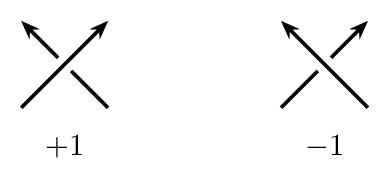
\includegraphics[width=.36\textwidth]{
knot-theory-assets/crossing-signs.png}
\end{center}
In words: turn the picture so that both
strands point upwards. The crossing is
positive when the over-strand goes from
the lower left to the upper right. This
is \cite[Definition 4.5.1]{murasugi}.
If the directions of both strands are
reversed, the sign does not change. If
the direction of only one strand is
reversed, the sign changes.

\medskip\noindent
Let $L$ be an oriented link with two
components $K_1$ and $K_2$, and let
$c_1,\ldots,c_m$ be the crossings of
$D$ where a strand of $K_1$ meets a
strand of $K_2$. Crossings of a
component with itself are not counted.
The {\it linking number} is
$$
\operatorname{lk}(K_1,K_2)
=
\frac{1}{2}
\sum_{i=1}^{m}
\operatorname{sign}(c_i).
$$

\begin{theorem}
\label{theorem-linking-number}
The linking number does not depend on
the diagram, so it is an invariant of
the oriented link. It is an integer and
$\operatorname{lk}(K_1,K_2)
=\operatorname{lk}(K_2,K_1)$.
\end{theorem}

\begin{proof}
See \cite[Theorem 4.5.1 and
Exercise 4.5.1]{murasugi}. The idea of
the first part: a move $R_1$ creates a
crossing of a component with itself,
which is not counted. A move $R_2$
creates two crossings of opposite
signs. A move $R_3$ moves the three
crossings without changing their signs.
\end{proof}

\begin{example}
\label{example-hopf-link}
The {\it Hopf link} is the link with
two components that has a diagram with
two crossings: two circles, each
passing once over and once under the
other. Orient it so that both crossings
are positive. Then the linking number
is $(1+1)/2=1$. For the trivial link
with two components there is a diagram
without crossings, so the linking
number is $0$. Hence the Hopf link is
not trivial. Reversing the direction of
one component of the Hopf link gives
linking number $-1$.
\end{example}

\noindent
The {\it writhe} $w(D)$ of a diagram
$D$ of an oriented link is the sum of
the signs of all crossings of $D$
(\cite[Definition 4.5.2]{murasugi},
where it is also called the Tait
number, and
\cite[Definition 3.4]{lickorish}).
The moves $R_2$ and $R_3$ do not change
$w(D)$, for the reasons given in the
proof of
Theorem \ref{theorem-linking-number}.
A move $R_1$ changes $w(D)$ by $+1$ or
$-1$, the sign of the crossing of the
kink. So the writhe is not an invariant
of the link; it is a property of the
diagram. For a knot, $w(D)$ does not
depend on the chosen direction, because
reversing it reverses both strands at
every crossing.

\section{Three-colourings}
\label{section-three-colourings}

\noindent
This invariant does not appear in the
course files that I read; it is in the
chapter of \cite{murasugi} on classical
invariants, and it is the fastest proof
that the trefoil is knotted.

\medskip\noindent
A diagram is {\it three-colourable} if
each of its arcs can be given one of
three colours so that at least two
colours are used and, at every
crossing, the three arcs that meet
there (the over-strand and the two
pieces of the under-strand) have either
all the same colour or three different
colours.

\begin{proposition}
\label{proposition-three-colourable}
If one diagram of a knot is
three-colourable, then every diagram of
that knot is three-colourable.
\end{proposition}

\begin{proof}
See \cite[Proposition 4.6.1]{murasugi};
one checks the three Reidemeister
moves.
\end{proof}

\noindent
The diagram of the unknot without
crossings has one arc, so it is not
three-colourable. The diagram of the
trefoil in
Section \ref{section-trefoil} has three
arcs, and at each crossing all three
meet; giving them three different
colours is a three-colouring. Hence the
trefoil is not equivalent to the
unknot. The usual diagram of the figure
eight knot is not three-colourable
\cite[Example 4.6.1]{murasugi}, so this
invariant does not tell the figure eight
knot from the unknot.

\section{The Kauffman bracket}
\label{section-kauffman-bracket}

\noindent
In this section diagrams are not
oriented. At a crossing there are two
ways to remove the crossing by
reconnecting the four ends, called the
two {\it smoothings}.
\begin{center}
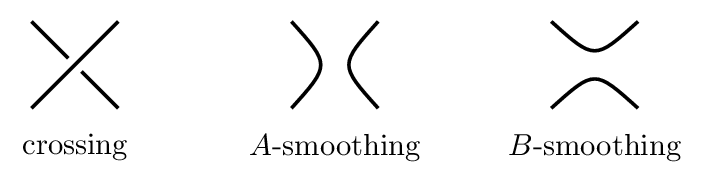
\includegraphics[width=.75\textwidth]{
knot-theory-assets/smoothings.png}
\end{center}
To tell them apart: turn the picture so
that the over-strand goes from the lower
left to the upper right. The
{\it $A$-smoothing} gives two vertical
pieces and the {\it $B$-smoothing} gives
two horizontal pieces. If the picture is
turned by a quarter of a turn, the names
$A$ and $B$ are exchanged, so the rule
needs the over-strand in the stated
position.

\medskip\noindent
The {\it Kauffman bracket} assigns to
each diagram $D$ a Laurent polynomial
$\langle D\rangle$ in one variable $A$
with integer coefficients. It is
determined by three rules
\cite[Definition 3.1]{lickorish}. Write
$O$ for the diagram of one circle
without crossings, and $D\sqcup O$ for
$D$ together with one more circle that
crosses nothing. Write $D_A$ and $D_B$
for the diagrams obtained from $D$ by
the $A$-smoothing and the $B$-smoothing
of one chosen crossing.
$$
\langle O\rangle=1,
$$
$$
\langle D\sqcup O\rangle
=(-A^{2}-A^{-2})\langle D\rangle,
$$
\begin{equation}
\label{equation-bracket-smoothing}
\langle D\rangle
=A\langle D_A\rangle
+A^{-1}\langle D_B\rangle.
\end{equation}
The bracket was introduced by Kauffman
\cite{kauffman-state-models}; see also
\cite[Theorem 11.4.1]{murasugi}.

\medskip\noindent
{\bf State sum.} Apply
(\ref{equation-bracket-smoothing}) to
every crossing. If $D$ has $n$
crossings, the result is a sum over the
$2^n$ ways of choosing a smoothing at
each crossing. Such a choice $s$ is a
{\it state}. After smoothing all
crossings there are no crossings left,
only a number $|s|$ of disjoint circles.
Let $a(s)$ be the number of
$A$-smoothings and $b(s)$ the number of
$B$-smoothings in $s$. Put
$$
d=-A^{2}-A^{-2}.
$$
A diagram of $|s|$ disjoint circles has
bracket $d^{|s|-1}$ by the first two
rules. Therefore
\begin{equation}
\label{equation-state-sum}
\langle D\rangle
=\sum_{s}A^{a(s)-b(s)}d^{|s|-1}.
\end{equation}
This formula shows that the three rules
do determine $\langle D\rangle$ and
that the order in which the crossings
are smoothed does not matter.

\begin{lemma}
\label{lemma-smoothing-sign}
At a positive crossing of an oriented
diagram, the $A$-smoothing is the one
that respects the directions of the
strands. At a negative crossing, the
$B$-smoothing is the one that respects
the directions.
\end{lemma}

\begin{proof}
Turn a positive crossing so that both
strands point upwards. By the
definition of the sign, the over-strand
goes from the lower left to the upper
right. The $A$-smoothing gives two
vertical pieces, and both can be
directed upwards, in agreement with the
four ends. The two horizontal pieces of
the $B$-smoothing cannot: the lower
piece would join two ends that both
point into the crossing. Now take a
negative crossing with both strands
pointing upwards. Its over-strand goes
from the lower right to the upper left.
Turning the picture by a quarter of a
turn puts the over-strand in the
standard position and exchanges
vertical and horizontal. So, in the
position with both strands pointing
upwards, the two vertical pieces are
the $B$-smoothing, and they are the
ones that respect the directions.
\end{proof}

\begin{lemma}
\label{lemma-bracket-kink}
Let $D$ be a diagram with a kink and
let $D'$ be the diagram without it. The
sign of the crossing of a kink does not
depend on the direction of travel. If
it is positive, then
$\langle D\rangle
=-A^{3}\langle D'\rangle$.
If it is negative, then
$\langle D\rangle
=-A^{-3}\langle D'\rangle$.
\end{lemma}

\begin{proof}
Both strands at the crossing of a kink
belong to the same piece of curve, so
reversing the direction reverses both
and the sign is unchanged. Suppose the
crossing is positive. The smoothing
that respects the directions cuts the
loop off as a separate circle; the
other smoothing leaves one strand
without a loop. By
Lemma \ref{lemma-smoothing-sign}
the first one is the $A$-smoothing. So
$$
\begin{aligned}
\langle D\rangle
&=A\langle D'\sqcup O\rangle
+A^{-1}\langle D'\rangle\\
&=\left(A(-A^{2}-A^{-2})+A^{-1}\right)
\langle D'\rangle\\
&=-A^{3}\langle D'\rangle.
\end{aligned}
$$
For a negative crossing the roles of
$A$ and $A^{-1}$ are exchanged. This is
\cite[Lemma 3.2]{lickorish}.
\end{proof}

\begin{lemma}
\label{lemma-bracket-r2-r3}
The moves $R_2$ and $R_3$ do not change
the Kauffman bracket.
\end{lemma}

\begin{proof}
See \cite[Lemma 3.3]{lickorish}. For
$R_2$ one applies
(\ref{equation-bracket-smoothing}) to
the two crossings. Of the four terms,
one contains a small circle and carries
the factor $d$; the value
$d=-A^{2}-A^{-2}$ is exactly the one
that makes three of the four terms
cancel. The move $R_3$ follows from
$R_2$.
\end{proof}

\noindent
So the bracket fails to be an invariant
of links only because of the move
$R_1$, and
Lemma \ref{lemma-bracket-kink} says
precisely how it fails.

\section{The Jones polynomial}
\label{section-jones-polynomial}

\noindent
The writhe fails to be invariant in the
same way as the bracket: only under
$R_1$, and by a controlled amount. The
two failures cancel.

\begin{theorem}
\label{theorem-jones-invariant}
Let $D$ be a diagram of an oriented
link $L$. The Laurent polynomial
$$
(-A)^{-3w(D)}\langle D\rangle
$$
does not depend on the diagram $D$ of
$L$. Here $\langle D\rangle$ is the
bracket of $D$ with the directions
forgotten.
\end{theorem}

\begin{proof}
By Theorem \ref{theorem-reidemeister}
it is enough to check the three moves.
The moves $R_2$ and $R_3$ change neither
$w(D)$ nor $\langle D\rangle$, by
Section \ref{section-linking-number}
and Lemma \ref{lemma-bracket-r2-r3}.
Let $D$ have one more kink than $D'$,
with positive crossing. Then
$w(D)=w(D')+1$ and, by
Lemma \ref{lemma-bracket-kink},
$\langle D\rangle
=-A^{3}\langle D'\rangle$.
Since $(-A)^{-3}=-A^{-3}$,
$$
\begin{aligned}
(-A)^{-3w(D)}\langle D\rangle
&=(-A)^{-3w(D')}(-A^{-3})(-A^{3})
\langle D'\rangle\\
&=(-A)^{-3w(D')}\langle D'\rangle.
\end{aligned}
$$
The case of a negative kink is the
same with $A^{-1}$ in place of $A$.
This is \cite[Theorem 3.5]{lickorish}
and \cite[Theorem 11.4.2]{murasugi}.
\end{proof}

\noindent
The {\it Jones polynomial} $V(L)$ of an
oriented link $L$ is the polynomial of
Theorem \ref{theorem-jones-invariant}
after the substitution
$A=t^{-1/4}$
(\cite[Definition 3.6]{lickorish}):
\begin{equation}
\label{equation-jones-definition}
V(L)=
(-A)^{-3w(D)}\langle D\rangle,
\quad
t=A^{-4}.
\end{equation}
It is a Laurent polynomial in
$t^{1/2}$. It was found by Jones
\cite{jones-polynomial} by a different
route. The polynomial
$(-A^{3})^{-w(D)}\langle D\rangle$
before the substitution is called the
$X$ polynomial in
\cite[Section 6.1]{adams-knot-book};
this is the ``polinomio $X$'' of my
exercise sheet {\tt Ejercicios.pdf}.

\medskip\noindent
{\bf First properties.}
\begin{enumerate}
\item The unknot has $V=1$.
\item Adding a separate unknotted
circle multiplies $V$ by
$d=-t^{1/2}-t^{-1/2}$. So the trivial
link with $c$ components has
$V=(-t^{1/2}-t^{-1/2})^{c-1}$.
\item Reversing the directions of all
components changes no sign of crossing,
so $V$ does not change. In particular
$V(K)$ of a knot $K$ does not depend on
a direction of $K$.
\item Let $L^{\circ}$ be obtained from
$L$ by reversing the direction of one
component $K$, and let $\lambda$ be the
sum of the linking numbers of $K$ with
the other components. The bracket is
the same. The crossings between $K$
and the rest change sign, and their
signs add up to $2\lambda$, so
$w$ decreases by $4\lambda$. Then
$(-A)^{-3w}$ is multiplied by
$(-A)^{12\lambda}=t^{-3\lambda}$ and
$$
V(L^{\circ})=t^{-3\lambda}V(L).
$$
This is stated in
\cite[p.\ 26]{lickorish}.
\end{enumerate}
Items (3) and (4) answer questions 3
and 4 of {\tt Ejercicios.pdf}.

\begin{proposition}[Skein relation]
\label{proposition-jones-skein}
Let $L_{+}$, $L_{-}$ and $L_{0}$ be
oriented links with diagrams that are
equal outside a small disc, where
$L_{+}$ has a positive crossing,
$L_{-}$ has a negative crossing and
$L_{0}$ has the smoothing that respects
the directions. Then
$$
t^{-1}V(L_{+})-tV(L_{-})
+(t^{-1/2}-t^{1/2})V(L_{0})=0.
$$
\end{proposition}

\begin{proof}
See \cite[Proposition 3.7]{lickorish}.
One writes
(\ref{equation-bracket-smoothing}) for
the positive and for the negative
crossing and eliminates the smoothing
that does not respect the directions.
\end{proof}

\begin{proposition}
\label{proposition-jones-at-one}
Let $L$ be an oriented link with $c$
components. Setting $t^{1/2}=1$ in
$V(L)$ gives $(-2)^{c-1}$.
\end{proposition}

\begin{proof}
This is question 2 of
{\tt Ejercicios.pdf}. Set $t^{1/2}=1$
in
Proposition \ref{proposition-jones-skein}.
The third term disappears, and the
relation says that the value is the same
for $L_{+}$ and $L_{-}$. So the value
does not change when a crossing of a
diagram is switched. Any diagram becomes
a diagram of a trivial link after
switching some crossings (a standard
fact, not proved here). For the trivial
link with $c$ components the value is
$(-1-1)^{c-1}$ by property (2).
\end{proof}

\section{The trefoil}
\label{section-trefoil}

\noindent
Let $n\geq 1$. Let $D_n$ be the
following diagram: two strands that
cross $n$ times, one crossing above the
other, closed up by two arcs on the
right. The picture shows $D_3$ with its
crossings $c_1$, $c_2$, $c_3$.
\begin{center}
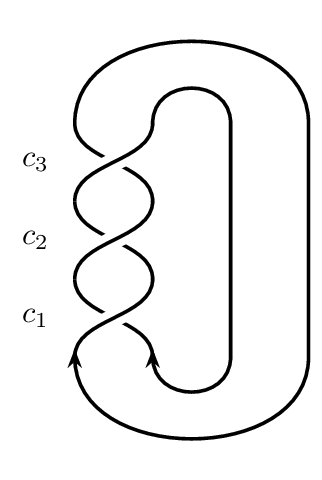
\includegraphics[width=.3\textwidth]{
knot-theory-assets/trefoil-braid.png}
\end{center}
Both strands are directed upwards
through the crossings, and at every
crossing the over-strand goes from the
lower left to the upper right. So all
$n$ crossings are positive and
$$
w(D_n)=n.
$$
The {\it right-handed trefoil} is the
knot with diagram $D_3$. The diagram
$D_2$ is a diagram of the Hopf link of
Example \ref{example-hopf-link}, and
$D_1$ is a circle with one positive
kink. Following a strand upwards, it
changes side at each crossing; so $D_n$
has one component when $n$ is odd and
two components when $n$ is even.

\medskip\noindent
{\bf The states of $D_n$.} At each
crossing the over-strand is in the
standard position, so the
$A$-smoothing gives two vertical pieces
and the $B$-smoothing gives two
horizontal pieces: a cap below and a
cup above. Let $s$ be a state with $k$
horizontal smoothings.
\begin{enumerate}
\item If $k=0$, all smoothings are
vertical, and what remains is two
circles, one inside the other. So
$|s|=2$.
\item If $k\geq 1$, the $k$ horizontal
smoothings cut the picture into $k$
pieces, going around: from the cup of
one horizontal smoothing, up through
the vertical smoothings, to the cap of
the next horizontal smoothing. After
the last one the piece continues
through the two closing arcs to the
first one. Each piece is one circle. So
$|s|=k$.
\end{enumerate}
There are $\binom{n}{k}$ states with
$k$ horizontal smoothings, and each has
$a(s)-b(s)=n-2k$. By
(\ref{equation-state-sum}),
\begin{equation}
\label{equation-bracket-dn}
\langle D_n\rangle
=A^{n}d
+\sum_{k=1}^{n}\binom{n}{k}
A^{n-2k}d^{k-1}.
\end{equation}

\medskip\noindent
{\bf The bracket of $D_3$.} For $n=3$
there are $8$ states.
\begin{center}
\begin{tabular}{c|c|c|c}
$k$ & states & circles & contribution
\\
\hline
$0$ & $1$ & $2$ & $A^{3}d$ \\
$1$ & $3$ & $1$ & $3A$ \\
$2$ & $3$ & $2$ & $3A^{-1}d$ \\
$3$ & $1$ & $3$ & $A^{-3}d^{2}$
\end{tabular}
\end{center}
Expand each contribution, using
$d=-A^{2}-A^{-2}$ and
$d^{2}=A^{4}+2+A^{-4}$.
$$
\begin{aligned}
A^{3}d&=-A^{5}-A,\\
3A&=3A,\\
3A^{-1}d&=-3A-3A^{-3},\\
A^{-3}d^{2}&=A+2A^{-3}+A^{-7}.
\end{aligned}
$$
Add them up, power by power. The
coefficient of $A^{5}$ is $-1$. The
coefficient of $A$ is $-1+3-3+1=0$. The
coefficient of $A^{-3}$ is $-3+2=-1$.
The coefficient of $A^{-7}$ is $1$.
Hence
\begin{equation}
\label{equation-bracket-trefoil}
\langle D_3\rangle
=-A^{5}-A^{-3}+A^{-7}.
\end{equation}
This agrees with the bracket of the
trefoil diagram computed in
\cite[p.\ 25]{lickorish}.

\medskip\noindent
{\bf The Jones polynomial.} We have
$w(D_3)=3$ and
$(-A)^{-9}=-A^{-9}$. By
(\ref{equation-jones-definition}),
$$
\begin{aligned}
V
&=-A^{-9}
\left(-A^{5}-A^{-3}+A^{-7}\right)\\
&=A^{-4}+A^{-12}-A^{-16}.
\end{aligned}
$$
With $t=A^{-4}$ this is the Jones
polynomial of the right-handed trefoil:
\begin{equation}
\label{equation-jones-trefoil}
V=t+t^{3}-t^{4}.
\end{equation}
It agrees with
\cite[Example 11.1.1]{murasugi}. Two
checks: at $t=1$ the value is
$1+1-1=1$, as
Proposition \ref{proposition-jones-at-one}
demands for a knot; and $V\neq 1$, so
the trefoil is not the unknot.

\medskip\noindent
{\bf A second way.} Apply
(\ref{equation-bracket-smoothing}) only
to the top crossing of $D_n$. The
$A$-smoothing gives $D_{n-1}$. The
$B$-smoothing gives a single closed
curve on which the other $n-1$
crossings have become kinks, which can
be removed one after the other starting
from the top. On this curve one of the
two strands is travelled downwards, so
each of these crossings is now
negative, and by
Lemma \ref{lemma-bracket-kink} the
curve has bracket $(-A^{-3})^{n-1}$.
Hence
$$
\langle D_n\rangle
=A\langle D_{n-1}\rangle
+A^{-1}(-A^{-3})^{n-1}.
$$
Starting from
$\langle D_1\rangle=-A^{3}$:
$$
\begin{aligned}
\langle D_2\rangle
&=A(-A^{3})+A^{-1}(-A^{-3})\\
&=-A^{4}-A^{-4},\\
\langle D_3\rangle
&=A(-A^{4}-A^{-4})+A^{-1}A^{-6}\\
&=-A^{5}-A^{-3}+A^{-7}.
\end{aligned}
$$
The value of $\langle D_2\rangle$ is
the bracket of the Hopf link diagram in
\cite[p.\ 24]{lickorish}, and
$\langle D_3\rangle$ agrees with
(\ref{equation-bracket-trefoil}).

\begin{proposition}
\label{proposition-jones-two-n}
For every $n\geq 1$,
$$
d\,\langle D_n\rangle
=(-A^{-3})^{n}+A^{n}(d^{2}-1).
$$
For $n$ odd, the knot with diagram
$D_n$ has Jones polynomial
$$
V=
t^{(n-1)/2}\,
\frac{1+t+t^{2}-t^{n+1}}{1+t}.
$$
\end{proposition}

\begin{proof}
If the term $k=0$ of
(\ref{equation-bracket-dn}) were
$A^{n}d^{-1}$ instead of $A^{n}d$, the
sum would be the binomial expansion of
$d^{-1}(A+A^{-1}d)^{n}$. Now
$$
A+A^{-1}d=A-A-A^{-3}=-A^{-3}.
$$
So
$$
\langle D_n\rangle
=d^{-1}(-A^{-3})^{n}
+A^{n}(d-d^{-1}),
$$
which is the first formula. For the
second, let $n$ be odd, so that
$(-A^{-3})^{n}=-A^{-3n}$ and
$V=-A^{-3n}\langle D_n\rangle$. In
terms of $t=A^{-4}$ we have
$A^{-6n}=t^{3n/2}$,
$A^{-2n}=t^{n/2}$,
$d=-t^{-1/2}(1+t)$ and
$d^{2}-1=t^{-1}(1+t+t^{2})$. Then
$$
\begin{aligned}
d\,V
&=-A^{-3n}
\left(-A^{-3n}+A^{n}(d^{2}-1)\right)\\
&=A^{-6n}-A^{-2n}(d^{2}-1)\\
&=t^{3n/2}-t^{n/2-1}(1+t+t^{2}),
\end{aligned}
$$
and dividing by $d=-t^{-1/2}(1+t)$
gives the formula.
\end{proof}

\noindent
For $n=3$ the formula gives
$t(1+t+t^{2}-t^{4})/(1+t)
=t(1+t^{2}-t^{3})$, which is
(\ref{equation-jones-trefoil}). For
$n=5$ it gives
$t^{2}+t^{4}-t^{5}+t^{6}-t^{7}$.
The knot with diagram $D_n$ is the
torus knot of type $(2,n)$ of
Section \ref{section-torus-knots}, so
this answers question 1 of
{\tt Ejercicios.pdf}.
The script
{\tt scripts/check\_knot\_jones.py}
computes the bracket of $D_n$ for
$n\leq 10$ by brute force over all
states and confirms
(\ref{equation-bracket-dn}), the
recursion,
Proposition \ref{proposition-jones-two-n}
and
(\ref{equation-jones-trefoil}). It also
recomputes the trefoil from the diagram
of the knot tables, which is the
left-handed one.

\section{Mirror images and chirality}
\label{section-chirality}

\noindent
The {\it mirror image} $K^{*}$ of a
knot $K$ is its image under the
reflection $(x,y,z)\mapsto(x,y,-z)$.
A diagram of $K^{*}$ is obtained from a
diagram of $K$ by switching every
crossing. A knot is
{\it amphicheiral} if it is equivalent
to its mirror image, and {\it chiral}
otherwise. The reflection reverses the
orientation of $\mathbb{R}^3$, so it is
not allowed in the definition of
equivalence; this is why the question
makes sense. The image of $K$ under any
orientation-reversing homeomorphism is
equivalent to $K^{*}$. The first
problems of my file
{\tt Quiralidad y cubrientes
ramificados.pdf} are about such a
reflection, extended to
$S^3=\mathbb{R}^3\cup\{\infty\}$.

\begin{proposition}
\label{proposition-jones-mirror}
For every oriented link $L$, the Jones
polynomial of the mirror image $L^{*}$
is obtained by replacing $t$ by
$t^{-1}$ in the Jones polynomial of
$L$.
\end{proposition}

\begin{proof}
Switching all crossings exchanges the
$A$-smoothing and the $B$-smoothing at
every crossing, so by
(\ref{equation-state-sum}) the bracket
of the mirror diagram is obtained by
exchanging $A$ and $A^{-1}$. It also
changes the sign of every crossing, so
$w$ becomes $-w$. Hence the whole
expression
(\ref{equation-jones-definition})
changes by exchanging $A$ and $A^{-1}$,
that is, $t$ and $t^{-1}$. See
\cite[Chapter 11, Section 2]{murasugi}.
\end{proof}

\begin{example}
\label{example-trefoil-chiral}
The {\it left-handed trefoil} is the
mirror image of the right-handed one.
By (\ref{equation-jones-trefoil}) and
Proposition \ref{proposition-jones-mirror}
its Jones polynomial is
$t^{-1}+t^{-3}-t^{-4}$. This is
different from $t+t^{3}-t^{4}$, so the
two trefoils are not equivalent: the
trefoil is chiral
\cite[Example 11.2.1]{murasugi}.
The {\it figure eight knot} is the knot
with four crossings listed as $4_1$ in
the knot tables. Its Jones polynomial
is
$$
t^{-2}-t^{-1}+1-t+t^{2}
$$
(\cite[Table 3.1]{lickorish}, and the
script). It is unchanged by
$t\mapsto t^{-1}$, as it must be,
because the figure eight knot is
amphicheiral \cite[p.\ 43]{murasugi}.
\end{example}

\noindent
The linking number, the
three-colourings and the knot group of
Section \ref{section-knot-group} cannot
detect chirality. The Jones polynomial
can.

\section{Curves on the torus}
\label{section-curves-on-torus}

\noindent
The {\it torus} is
$T=S^1\times S^1$. We use
$S^1=\mathbb{R}/\mathbb{Z}$, so that
$T=\mathbb{R}^2/\mathbb{Z}^2$ is the
square $[0,1]\times[0,1]$ with opposite
sides glued. Its fundamental group is
abelian and
$$
\pi_1(T)=H_1(T;\mathbb{Z})
=\mathbb{Z}^2.
$$
The class of a loop
$\gamma=(\gamma_1,\gamma_2)$ in $T$ is
the pair of integers $(p,q)$, where $p$
is the number of times $\gamma_1$ goes
around the first circle and $q$ the
number of times $\gamma_2$ goes around
the second one. These are the
{\it winding numbers} of $\gamma$.

\medskip\noindent
For integers $p$ and $q$, not both
zero, the {\it linear loop} of class
$(p,q)$ is
$$
\gamma_{p,q}(s)=(ps,qs),
\quad 0\leq s\leq 1,
$$
read modulo $\mathbb{Z}^2$. On the
square it is a family of parallel
segments of slope $q/p$. The picture
shows $\gamma_{2,3}$.
\begin{center}
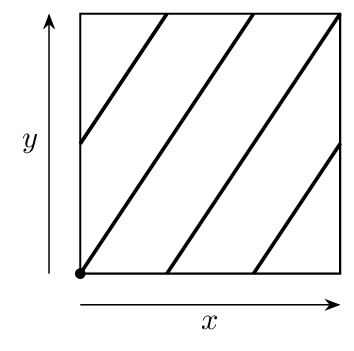
\includegraphics[width=.34\textwidth]{
knot-theory-assets/torus-square.png}
\end{center}

\begin{lemma}
\label{lemma-linear-loop-embedded}
The loop $\gamma_{p,q}$ has no
self-intersections if and only if
$\gcd(p,q)=1$. If $\gcd(p,q)=g$, the
loop runs $g$ times around the image of
$\gamma_{p/g,q/g}$.
\end{lemma}

\begin{proof}
We have
$\gamma_{p,q}(s)=\gamma_{p,q}(s')$ if
and only if both $p(s-s')$ and
$q(s-s')$ are integers. Suppose
$\gcd(p,q)=1$ and choose integers $u$
and $v$ with $up+vq=1$. Then
$$
s-s'=u\,p(s-s')+v\,q(s-s')
$$
is an integer, so $s$ and $s'$ are the
same point of the circle
$\mathbb{R}/\mathbb{Z}$. Conversely, if
$g=\gcd(p,q)>1$, then
$\gamma_{p,q}(s+1/g)=\gamma_{p,q}(s)$,
and
$\gamma_{p,q}(s)=\gamma_{p/g,q/g}(gs)$.
\end{proof}

\begin{proposition}
\label{proposition-simple-curves-torus}
The homotopy classes of oriented simple
closed curves in $T$ that are not
contractible correspond bijectively to
the pairs $(p,q)$ in $\mathbb{Z}^2$
with $\gcd(p,q)=1$. Here
$\gcd(0,\pm 1)=\gcd(\pm 1,0)=1$.
\end{proposition}

\begin{proof}
See
\cite[Proposition 1.5]{farb-margalit}.
Lemma \ref{lemma-linear-loop-embedded}
gives a curve for each such pair.
\end{proof}

\begin{remark}
\label{remark-winding-vector}
The same definition works for the
torus $(S^1)^n$ of any dimension: a
loop
$\gamma=(\gamma_1,\ldots,\gamma_n)$
has a winding number for each
coordinate, and the resulting
{\it winding vector} in
$\mathbb{Z}^n=H_1((S^1)^n;\mathbb{Z})$
is its homology class. The class
$(p,q)$ of a torus knot is the case
$n=2$. This is the vector that appears
for Lagrangian tori: if $L$ is a
Lagrangian torus in a symplectic
manifold $X$ and $u$ is a disc in $X$
with boundary on $L$, the boundary of
$u$ is a loop on $L$, and its winding
vector is the image of the class of $u$
under the boundary map
$H_2(X,L)\to H_1(L)=\mathbb{Z}^n$. For
the product torus
$\{|z_1|=\cdots=|z_n|=1\}$ in
$\mathbb{C}^n$, the unit disc in the
$i$-th coordinate, with the other
coordinates fixed, has winding vector
the $i$-th basis vector.
\end{remark}

\section{Torus knots}
\label{section-torus-knots}

\noindent
Write the three-sphere as
$$
S^3=\{(z,w)\in\mathbb{C}^2:
|z|^{2}+|w|^{2}=1\}.
$$
Consider the two pieces
$$
\begin{aligned}
A&=\{(z,w)\in S^3:|z|^{2}\leq 1/2\},\\
B&=\{(z,w)\in S^3:|w|^{2}\leq 1/2\}.
\end{aligned}
$$
This is the decomposition of the typed
note {\tt Toros y S3.pdf}, which writes
$z=x+iy$ and $w=u+iv$ and leaves the
following as things to convince oneself
of.
\begin{enumerate}
\item $S^3=A\cup B$, because $|z|^{2}$
and $|w|^{2}$ add up to $1$, so one of
them is at most $1/2$.
\item $A\cap B$ is the torus
$T=\{|z|=|w|=1/\sqrt{2}\}$.
\item $A$ and $B$ are {\it solid tori},
that is, homeomorphic to
$D^2\times S^1$, where $D^2$ is the
closed disc. For $A$ a homeomorphism
is $(z,w)\mapsto(\sqrt{2}z,w/|w|)$; on
$A$ we have $|w|^{2}\geq 1/2$, so
$w\neq 0$.
\end{enumerate}
The circle $\{z=0\}$ is the {\it core}
of $A$, and $\{w=0\}$ is the core of
$B$. A circle on $T$ on which $w$ is
constant bounds a disc in $A$ (let $z$
shrink to $0$) and is parallel to the
core of $B$. A circle on $T$ on which
$z$ is constant bounds a disc in $B$
and is parallel to the core of $A$. So
the two directions of $T$ exchange
their roles between $A$ and $B$
\cite[Proposition 7.2.3]{murasugi}.
The same note recalls the analogous
fact one dimension down: two discs
glued along their boundaries give a
sphere.

\medskip\noindent
Let $p$ and $q$ be integers with
$\gcd(p,q)=1$. The {\it torus knot}
$T(p,q)$ is the image in $S^3$ of the
linear loop of class $(p,q)$ on $T$:
$$
s\mapsto\frac{1}{\sqrt{2}}
\left(e^{2\pi ips},e^{2\pi iqs}\right),
\quad 0\leq s\leq 1.
$$
By
Lemma \ref{lemma-linear-loop-embedded}
it is a knot. If $\gcd(p,q)=g>1$, one
takes instead $g$ parallel copies of
the curve of class $(p/g,q/g)$; this is
a link with $g$ components, a
{\it torus link}.

\begin{remark}
\label{remark-murasugi-torus-notation}
In
\cite[Chapter 7, Section 1]{murasugi}
the torus link $K_{q,r}$ is built from
a cylinder with $r$ vertical segments,
by turning the top by the angle
$2\pi q/r$ and gluing top to bottom.
That $K_{q,r}$ has $\gcd(q,r)$
components is
\cite[Exercise 7.1.1]{murasugi}, which
was my Ejercicio 2 of Seminario de
Topolog\'ia B. The argument of my
solution: the segment that starts at
the point number $k$ ends at the point
number $k+q$ modulo $r$, so the
components are the orbits of
$k\mapsto k+q$ on
$\mathbb{Z}/r\mathbb{Z}$, and there are
$\gcd(q,r)$ of them. The knot $K_{q,r}$
goes $r$ times around the cylinder
direction and $q$ times around the
other one, so it is $T(q,r)$ or its
mirror image. I did not check which;
with the usual orientation of $S^3$ it
should be $T(q,r)$ for positive $q$ and
$r$. With $r=2$ the cylinder has two
strands with $q$ half turns, which is
the diagram $D_q$ of
Section \ref{section-trefoil} or its
mirror image; and
\cite[Example 7.1.1]{murasugi} states
that $K(3,2)$ is the right-handed
trefoil.
\end{remark}

\begin{theorem}
\label{theorem-torus-symmetry}
Let $\gcd(p,q)=1$.
\begin{enumerate}
\item $T(p,q)$ is equivalent to
$T(q,p)$.
\item $T(-p,-q)$ is the same subset as
$T(p,q)$, travelled in the opposite
direction.
\item $T(p,-q)$ is equivalent to the
mirror image of $T(p,q)$.
\item If $p$ or $q$ is $0$, $1$ or
$-1$, then $T(p,q)$ is the unknot.
\end{enumerate}
\end{theorem}

\begin{proof}
(1) The map $(z,w)\mapsto(w,z)$ of
$S^3$ sends $T(p,q)$ to $T(q,p)$. It is
the restriction of a linear map of
$\mathbb{R}^4$ that exchanges two pairs
of coordinates, so it has determinant
$1$ and preserves orientation.
(2) We have
$\gamma_{-p,-q}(s)=\gamma_{p,q}(1-s)$.
(3) The map
$(z,w)\mapsto(z,\overline{w})$ sends
$T(p,q)$ to $T(p,-q)$ and has
determinant $-1$, so it reverses
orientation.
(4) See
\cite[Proposition 7.2.1]{murasugi}. For
instance, on $T(1,q)$ the argument of
$z$ takes each value once. So $T(1,q)$
meets once each of the discs of $B$ on
which the argument of $z$ is constant,
and it can be pushed along these discs
to the core of $B$, which is a round
circle.
The statements (1) and (3) are
\cite[Theorem 7.2.4 and
Proposition 7.2.1]{murasugi}.
\end{proof}

\begin{theorem}[Classification of torus
knots]
\label{theorem-torus-classification}
Let $p,q,p',q'$ be integers different
from $0$, $1$ and $-1$, with
$\gcd(p,q)=\gcd(p',q')=1$. Then
$T(p,q)$ and $T(p',q')$ are equivalent
if and only if the set $\{p',q'\}$ is
equal to $\{p,q\}$ or to $\{-p,-q\}$.
In particular $T(p,q)$ is not
equivalent to its mirror image
$T(p,-q)$.
\end{theorem}

\begin{proof}
Not proved here. See
\cite[Theorem 7.4.3]{murasugi}. For
positive numbers the proof there
compares Alexander polynomials
(Section \ref{section-alexander}); the
chirality comes from the signature
\cite[Theorem 7.4.2]{murasugi}. For
positive numbers another proof, by the
knot group, is in
\cite[Example 1.24]{hatcher}.
\end{proof}

\begin{example}
\label{example-small-torus-knots}
$T(2,3)$ is a trefoil; by
Theorem \ref{theorem-torus-symmetry} it
is also $T(3,2)$. The knots $T(2,n)$
for odd $n$ are, up to mirror image,
the knots with diagram $D_n$ of
Proposition \ref{proposition-jones-two-n}.
The first torus knot that is not of
this kind is $T(3,4)$.
\end{example}

\begin{remark}
\label{remark-torus-knot-singularity}
The knot $T(p,q)$ lies on the complex
curve $\{z^{q}=w^{p}\}$, because
$(e^{2\pi ips})^{q}
=(e^{2\pi iqs})^{p}$.
More precisely, for $p,q\geq 1$ coprime
there are unique positive numbers
$r_1,r_2$ with $r_1^{q}=r_2^{p}$ and
$r_1^{2}+r_2^{2}=1$, and the
intersection of the curve
$\{z^{q}=w^{p}\}$ with $S^3$ is the
image of
$s\mapsto(r_1e^{2\pi ips},
r_2e^{2\pi iqs})$. Indeed, let
$z=r_1e^{2\pi ia}$ and
$w=r_2e^{2\pi ib}$ with $qa-pb$ an
integer, and let $up+vq=1$. Then
$s=ua+vb$ satisfies
$ps-a=-v(qa-pb)$ and
$qs-b=u(qa-pb)$, which are integers.
This curve is $T(p,q)$ drawn on a
parallel torus. So a trefoil is the
intersection of the cusp
$\{z^{3}=w^{2}\}$ with the sphere
around its singular point.
\end{remark}

\section{The knot group}
\label{section-knot-group}

\noindent
The {\it knot group} of a knot $K$ is
the fundamental group of its
complement,
$$
G(K)=\pi_1(S^3\setminus K).
$$
An equivalence of knots is a
homeomorphism of $S^3$ that maps one
complement onto the other, so
equivalent knots have isomorphic
groups. The same holds for a knot and
its mirror image. The unknot is the
core $\{w=0\}$ of $B$. Its complement
deformation retracts onto $A$, and then
onto the core of $A$, a circle. So the
group of the unknot is $\mathbb{Z}$.

\medskip\noindent
{\bf Van Kampen's theorem.} A typed
note of the course, the file
{\tt Sobre el teorema de Van
Kampen.pdf}, states it in the following
form. Let $X$ be the union of two open
path-connected sets $U_1$ and $U_2$
whose intersection is non-empty and
path-connected. Suppose
$$
\begin{aligned}
\pi_1(U_1)
&=\langle x\mid r\rangle,\\
\pi_1(U_2)
&=\langle y\mid s\rangle,\\
\pi_1(U_1\cap U_2)
&=\langle z\mid t\rangle,
\end{aligned}
$$
where $x$, $y$, $z$ stand for sets of
generators and $r$, $s$, $t$ for sets
of relations. Then $\pi_1(X)$ has a
presentation whose generators are those
of $x$ and $y$ together, and whose
relations are those of $r$ and $s$
together with one new relation for each
generator $z_k$ of $z$: the image of
$z_k$ in $\pi_1(U_1)$ is equal to the
image of $z_k$ in $\pi_1(U_2)$. The
general statement is
\cite[Theorem 1.20]{hatcher}. The
example of the note is the torus: $U_1$
is the square without its centre, with
free group on the two sides $a$ and
$b$; $U_2$ is a disc around the centre;
the loop around the centre becomes
$aba^{-1}b^{-1}$ in $U_1$ and is
trivial in $U_2$; so
$\pi_1(T)=\langle a,b\mid
aba^{-1}b^{-1}\rangle=\mathbb{Z}^2$.

\begin{theorem}
\label{theorem-torus-knot-group}
For $\gcd(p,q)=1$ and $p,q\geq 1$,
$$
G(T(p,q))
=\langle a,b\mid a^{p}=b^{q}\rangle.
$$
\end{theorem}

\begin{proof}
A sketch; the details are in
\cite[Example 1.24]{hatcher}. Let
$K=T(p,q)$ and cover $S^3\setminus K$
by $A\setminus K$ and $B\setminus K$,
slightly enlarged to make them open.
The set $B\setminus K$ deformation
retracts onto the core of $B$, so its
group is $\mathbb{Z}$, with a generator
$a$. Likewise $A\setminus K$ has group
$\mathbb{Z}$ with generator $b$, the
core of $A$. The intersection
$T\setminus K$ is a band that runs
parallel to $K$, so its group is
$\mathbb{Z}$, generated by a loop
$\ell$ of class $(p,q)$ on $T$. In $B$
the first coordinate direction of $T$
is parallel to the core and the second
one is contractible, so $\ell$ becomes
$a^{p}$. In $A$ it is the other way
around, so $\ell$ becomes $b^{q}$. Van
Kampen's theorem gives the single
relation $a^{p}=b^{q}$.
\end{proof}

\noindent
For the trefoil the group is
$\langle a,b\mid a^{2}=b^{3}\rangle$.
It is not abelian: sending $a$ to the
transposition $(1\,2)$ and $b$ to the
cycle $(1\,2\,3)$ respects the
relation, since both sides go to the
identity, and gives a surjection onto
the symmetric group $S_3$. So the group
of the trefoil is not $\mathbb{Z}$, and
this is a second proof that the trefoil
is knotted. For $p,q\geq 2$,
\cite[Example 1.24]{hatcher} shows that
the group $\langle a,b\mid
a^{p}=b^{q}\rangle$ determines the set
$\{p,q\}$.

\medskip\noindent
{\bf The Wirtinger presentation.} For
any knot, a presentation of the group
can be read from an oriented diagram
with arcs $\alpha_1,\ldots,\alpha_n$.
There is one generator $x_i$ for each
arc: a loop that starts above the
diagram, goes down, passes once under
the arc $\alpha_i$, and returns. There
is one relation for each crossing: if
$\alpha_i$ is the over-strand and
$\alpha_j$, $\alpha_k$ are the two
pieces of the under-strand, the
relation is
$$
x_ix_jx_i^{-1}=x_k
$$
for a suitable order of $j$ and $k$
\cite[Section 1.2,
Exercise 22]{hatcher}.
Question 8 of {\tt Ejercicios.pdf} asks
for such presentations for the torus
knots of type $(p,2)$, the square knot,
the granny knot and the knot $8_{19}$.

\medskip\noindent
Two consequences. First, in an abelian
group the relation becomes $x_j=x_k$;
going along the knot, all generators
become equal, so the abelianisation of
every knot group is $\mathbb{Z}$. The
knot group is interesting only because
it is not abelian. Second, for the
diagram $D_3$ of the trefoil there are
three arcs and at each crossing all
three meet. The relations are
$x_1x_2x_1^{-1}=x_3$ and its two cyclic
permutations. Using the first to
eliminate $x_3$, the second,
$x_2x_3x_2^{-1}=x_1$, becomes
$x_2x_1x_2=x_1x_2x_1$. Writing $x=x_1$
and $y=x_2$,
$$
G=\langle x,y\mid xyx=yxy\rangle.
$$
(I did not check the order of $j$ and
$k$ against the directions on $D_3$;
the other order gives the same
presentation with $x$ and $y$
exchanged.) This agrees with
Theorem \ref{theorem-torus-knot-group}:
put $a=xyx$ and $b=xy$. Then
$$
b^{3}=(xyx)(yxy)=(xyx)(xyx)=a^{2},
$$
and conversely $x=b^{-1}a$ and
$y=a^{-1}b^{2}$.

\begin{remark}
\label{remark-colourings-and-group}
A three-colouring of a diagram is the
same as a homomorphism from the knot
group onto $S_3$ that sends every
Wirtinger generator to a transposition:
the three colours are the three
transpositions, and
$x_ix_jx_i^{-1}=x_k$ holds for
transpositions exactly when all three
are equal or all three are different.
\end{remark}

\section{The Alexander polynomial}
\label{section-alexander}

\noindent
The {\it Conway polynomial}
$\nabla_L(z)$ of an oriented link is
determined by two rules
\cite[Chapter 6, Section 2]{murasugi}:
the unknot has $\nabla=1$, and for
three links as in
Proposition \ref{proposition-jones-skein},
$$
\nabla_{L_{+}}(z)-\nabla_{L_{-}}(z)
=z\,\nabla_{L_{0}}(z).
$$
The {\it Alexander polynomial} is
$$
\Delta_L(t)
=\nabla_L\left(t^{1/2}-t^{-1/2}\right)
$$
by \cite[Theorem 6.2.1]{murasugi}. It
was originally defined in other ways,
for instance from a Seifert matrix or
from the knot group; that these agree,
and that the two rules are consistent,
is not proved here.

\begin{example}
\label{example-alexander-trefoil}
Apply the rule to a kink: $L_{+}$ and
$L_{-}$ are both the unknot and $L_{0}$
is the trivial link with two
components, so that link has
$\nabla=0$. Apply it to a crossing of
the Hopf link $D_2$: $L_{-}$ is the
trivial link and $L_{0}$ is the unknot,
so the Hopf link has $\nabla=z$. Apply
it to a crossing of the trefoil $D_3$:
$L_{-}$ is a diagram of the unknot
(switching one crossing of $D_3$ lets
two crossings cancel by a move $R_2$,
leaving $D_1$) and $L_{0}$ is $D_2$.
Hence
$$
\nabla=1+z\cdot z=1+z^{2},
$$
and, since
$(t^{1/2}-t^{-1/2})^{2}=t-2+t^{-1}$,
the trefoil has
$$
\Delta(t)=t-1+t^{-1}.
$$
\end{example}

\begin{example}
\label{example-alexander-figure-eight}
My notebook page
{\tt Ejercicio 1.pdf} (13th semester)
computes the Alexander polynomial of
the figure eight knot in the same way,
resolving first the knot, then a Hopf
link, then a diagram of the trivial
link, and finds
$$
\Delta(t)=-t^{-1}+3-t.
$$
It writes the rule as
$\Delta(L_{+})-\Delta(L_{-})
+(t^{1/2}-t^{-1/2})\Delta(L_{0})=0$,
which is the rule above with $z$
replaced by $-z$. In these two examples
only $z^{2}$ occurs in the answer, so
the sign makes no difference. The value
agrees with $\nabla=1-z^{2}$.
\end{example}

\begin{theorem}
\label{theorem-alexander-torus}
For $q,r\geq 1$ with $\gcd(q,r)=1$,
the Alexander polynomial of the torus
knot $T(q,r)$ is
$$
\Delta(t)=
t^{-(q-1)(r-1)/2}\,
\frac{(1-t)(1-t^{qr})}
{(1-t^{q})(1-t^{r})}.
$$
\end{theorem}

\begin{proof}
Not proved here. This is the case of
knots of
\cite[Theorem 7.3.2]{murasugi}, which
is stated there without a full proof.
\end{proof}

\noindent
For $(q,r)=(2,3)$ the fraction is
$$
\frac{(1-t)(1-t^{6})}
{(1-t^{2})(1-t^{3})}
=\frac{1+t^{3}}{1+t}
=1-t+t^{2},
$$
and multiplying by $t^{-1}$ gives
$t^{-1}-1+t$, in agreement with
Example \ref{example-alexander-trefoil}.
The highest power of $t$ in the
fraction is $(q-1)(r-1)$; comparing
these polynomials is how
\cite[Theorem 7.4.1]{murasugi} tells
the torus knots with positive $q$, $r$
apart. Unlike the Jones polynomial, the
Alexander polynomial is unchanged by
$t\mapsto t^{-1}$ and does not detect
chirality.

\section{What else is in the course
files}
\label{section-course-files}

\noindent
A list of the remaining topics, with
the file where each one appears, for
the day I want to come back to them.
Nothing here is developed.
\begin{enumerate}
\item {\it Seifert surfaces.} Every
oriented link is the boundary of a
connected orientable surface in
$\mathbb{R}^3$
\cite[Theorem 5.1.1]{murasugi}. My file
{\tt Quiralidad y cubrientes
ramificados.pdf} triangulates a surface
with boundary and has a photograph of a
paper model.
\item {\it Branched covers.} The title
of the same file announces them, and
its later pages glue two copies of a
triangulated surface. I read only part
of that file, and I have not checked a
reference for this construction.
\item {\it Three-manifolds.} The file
{\tt 3-variedades.pdf} has my solutions
on gluing two handlebodies (``cubos con
asas'') along their boundaries and on
$S^2\times S^1$. The decomposition
$S^3=A\cup B$ of
Section \ref{section-torus-knots} is
the simplest example.
\item {\it Rational tangles.} Ejercicios
9 to 12 and Tarea 10 of Seminario de
Topolog\'ia B are about Conway's
``dance'': two operations on tangles,
a twist $T$ and a rotation $R$, which
act on the fraction of the tangle. My
solution of Ejercicio 10 shows that
every rational number can be reached
and brought back to $0$. The formulas
for $T$ and $R$ are not in the files I
read; tangles are treated in
\cite{murasugi}.
\item {\it Graphs.} Questions 6 and 7 of
{\tt Ejercicios.pdf} relate the Tutte
polynomial of a plane graph to the
Kauffman bracket of the link diagram
built from its medial graph. The files
{\tt delta\_y\_Q.pdf} and
{\tt ejerciciospolinomios.pdf} are
about polynomials of ribbon graphs (the
operation $\delta(e)$ and the
topological transition polynomial $Q$).
\item {\it Homology.} The two files of
``Ejercicios de homolog\'ia'' are
exercises on simplicial homology
(tetrahedron, M\"obius band, projective
plane, torus) and relative homology.
\end{enumerate}


\bibliography{my}
\bibliographystyle{amsalpha}

\end{document}
